%!TEX root = ../thesis.tex
%%--------------------------------------------------------------------------
%% OPENSTACK AND DEVSTACK
%%--------------------------------------------------------------------------


In this chapter we are going to present OpenStack and DevStack giving a brief overview of them and focusing on their components and aspects that concern our thesis topic.

\section{OpenStack}
\label{sec:openstack}
OpenStack is an open-source cloud computing software platform that provides a complete IaaS solution for public and private clouds. Founded by Nasa\footnote{\url{www.nasa.gov} (2015)} and Rackspace Cloud\footnote{\url{www.rackspace.com} (2015)} in 2010 OpenStack is now one of the biggest open-source projects with more than twenty thousand people working on it and more than twenty million code lines. It is a cloud operating system that controls large pools of compute, storage, and networking resources throughout a datacenter, with the possibility to control all of them trough a dashboard and enabling enterprises and service providers to offer on-demand computing resources.\\
One of its main strengths is the modularity that provides the necessary flexibility to design different configuration for a cloud environment; its core components are:
\begin{description}
	\item[Compute] The service called \texttt{Nova} is the primary computing engine and it is used to deploy and manage large number of Virtual Machines.
	\item[Storage] The storage platform, divided in Object Storage (\texttt{Swift}) and Block Storage (\texttt{Cinder}).
	\item[Network] The service \texttt{Neutron} that offers Networking as a Service
	\item[Dashboard] The dashboard \texttt{Horizon} provides users with a graphical user interface to access, provision, and automate cloud-based resources.
	\item[Shared Services] Other services, that makes easier to manage the IaaS, such as the Identity Service (\texttt{Keystone}), the Image Service (\texttt{Glance}), Telemetry (\texttt{Ceilometer}), Orchestration (\texttt{Heat}) and others.
\end{description}

\begin{figure}[!ht]
\centering{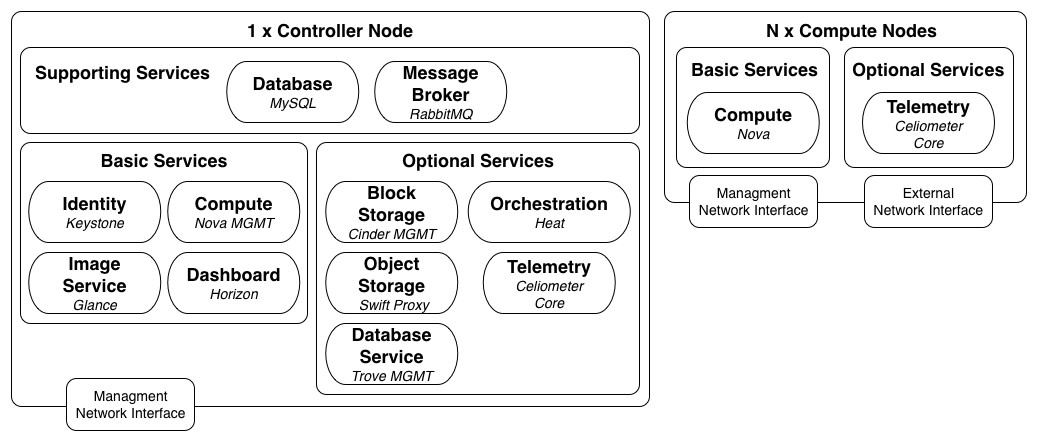
\includegraphics[width=\textwidth]{images/openstack_arch.png}}
\label{fig:openstack_1plusN}
\caption{A ``1 + N'' OpenStack configuration}
\end{figure}

We have decided to focus on the creation of a ``1 + N'' installation of OpenStack that is composed by one \textit{Controller} node and N \textit{Compute} nodes with legacy networking. Legacy networking refers to a basic solution in which we do not deploy \texttt{Neutron} but we exploit \code{nova-network}, a \texttt{Nova} service described in paragraph \ref{par:openstack_nova_net}. The figure~\ref{fig:openstack_1plusN} on page~\pageref{fig:openstack_1plusN} provides a high level view of all the OpenStack services, both basic and optional, that have to be installed both on the Controller and the Compute nodes to setup a ``1 + N'' configuration.\\ 
The Controller node is responsible for globally managing the cloud operations. It runs the user \texttt{Identity} service, the Virtual Machine \texttt{Image} service, the management portion of the \texttt{Compute} service, and a \textit{Dashboard} through which the users can request the creation of new Virtual Machines. Optionally, the node can run the management portions of the \texttt{Block}, \texttt{Object}, and \texttt{Database Storage} services, and the \texttt{Telemetry} and \texttt{Orchestration} services. The Controller node also runs a series of supporting services (i.e., the \texttt{Database} and \texttt{Message Broker} services). Each of the N basic Compute nodes, on the other hand, runs the \texttt{Compute} service and optionally the \texttt{Telemetry} service.

\subsection{Nova}
\label{sec:openstack_nova}
OpenStack Compute module, \texttt{Nova}, is the core of OpenStack; it takes care to deploy and manage Virtual Machines, place them on physical machines, let them communicate, store their informations on an SQL database and offers both a set of APIs reachable through HTTP requests and a command-line client.
In the next paragraphs we briefly describe the three \texttt{Nova} sub-modules that are relevant for our work.

\subparagraph{Nova-compute}
\label{par:openstack_nova_compute}
The \texttt{nova-compute} is the sub-module that takes care to boot, resize, live-migrate and destroy Virtual Machines running on physical server and let them communicate with the hypervisor.\\
Hereunder are reported four examples of the main commands (also accessible through the Nova APIs) used to boot, resize, destroy and live-migrate Virtual Machines:
\begin{itemize}
	\item \code{\$ nova boot --flavor <flavor> --image <image>}
	\item \code{\$ nova resize --flavor <vm> <flavor>}
	\item \code{\$ nova delete <vm>}
	\item \code{\$ nova live-migration <vm> <host>}
\end{itemize}

\subparagraph{Nova-network}
\label{par:openstack_nova_net}
\texttt{Nova-network} is the basic network management module of OpenStack included directly in \texttt{Nova}. Unlike \texttt{Neutron}, that is able to virtualize and manage both layer 2 (logical) and layer 3 (network) of the OSI network, \texttt{nova-network} provides only simple layer 3 virtualization and has some limitations on the network topology.\\
However \texttt{nova-network} is still supported by OpenStack and can powerful enough to support a ``1 + N'' configuration needed for our purposes. It also streamlines the installation process as it avoids having to install another service (\texttt{Neutron}) and its dependencies.

\subparagraph{Nova-scheduler}
\label{par:openstack_nova_sched}
\texttt{Nova} uses the \texttt{nova-scheduler} service to determine how to dispatch compute requests. It is used, for example, to determine on which host a Virtual Machine should launch. The system administrator can modify and configure the \code{/etc/nova/nova.conf} configuration file to adjust the criteria under which the \texttt{nova-scheduler} will make the Virtual Machines placement decisions. The process of placing Virtual Machines on the more suitable host is divided in a \textit{filtering} step where a list of candidate hosts is generated and a \textit{weighing} step where the list is ordered according to the selected criteria and the best host is chosen.

\section{DevStack}
\label{sec:devstack}

% - devstack
% 	- stack.sh
% 	- unstack.sh
% 	- clean.sh
% 	- 
% 	- configurations local.conf
 
DevStack\footnote{More info at \url{docs.openstack.org/developer/devstack}} is a set of scripts and utilities to quickly deploy an OpenStack cloud environment and it is freely available on GitHub\footnote{\url{github.com/openstack-dev/devstack}}.\\
DevStack allows developers and system administrators to automate the process of installing OpenStack on a server reducing it to a simple command for every installation.\\
The services that are configured by default are Identity (\texttt{Keystone}), Object Storage (\texttt{Swift}), Image Storage (\texttt{Glance}), Block Storage (\texttt{Cinder}), Compute (\texttt{Nova}), Network (\texttt{Nova}), Dashboard (\texttt{Horizon}) and Orchestration (\texttt{Heat}).
The main script is \code{stack.sh}; before installing OpenStack it takes care of installing all the required dependencies and setup the system to host the OpenStack installation. All the configuration can be achieved overriding environment variables used in \code{stack.sh} by creating the file \code{local.conf} with a \code{localrc} section as shown below:\\
\begin{lstlisting}[numbers=none]
[[local|localrc]]
VARIABLE=value
\end{lstlisting}
\\
